Um designer de jogos planeja um jogo que faz uso de um tabuleiro de dimens�o n x n, com $n \geq 2$, no qual cada jogador, na sua vez, coloca uma pe�a sobre uma das casas vazias do tabuleiro. Quando uma pe�a � posicionada, a regi�o formada pelas casas que est�o na mesma linha ou coluna dessa pe�a � chamada de zona de combate dessa pe�a. Na figura est� ilustrada a zona de combate de uma pe�a colocada em uma das casas de um tabuleiro de dimens�o 8 x 8. 

\begin{figure}[h]
\centering
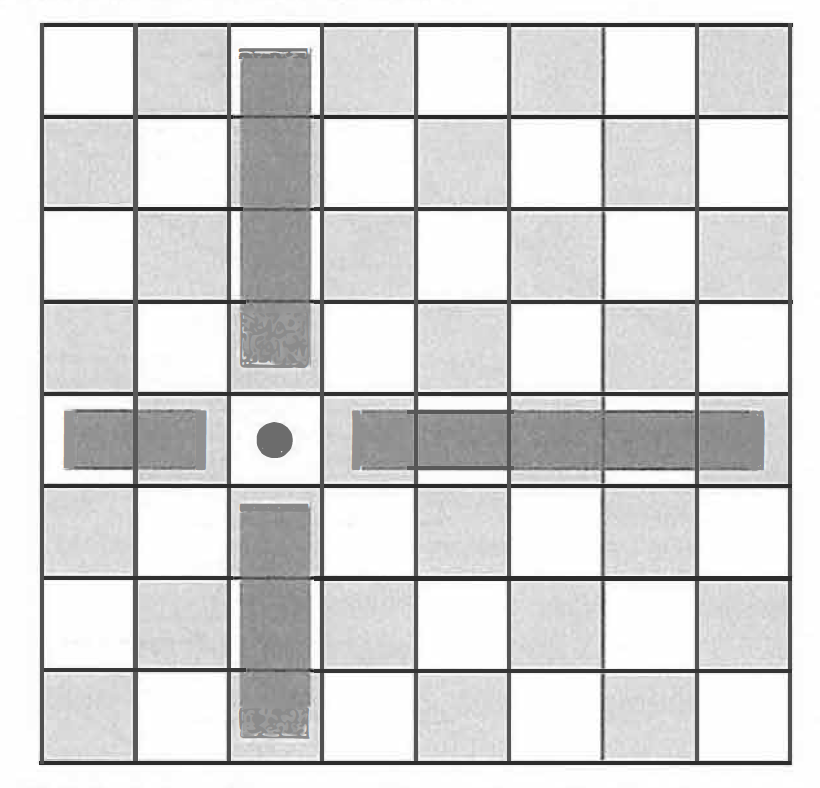
\includegraphics[width=8cm]{../figuras/q171-2018}
\end{figure}

O tabuleiro deve ser dimensionado de forma que a probabilidade de se posicionar a segunda pe�a aleatoriamente, seguindo a regra do jogo, e esta ficar 
sobre a zona de combate da primeira, seja inferior a $\frac 1 5$. 
A dimens�o m�nima que o designer deve adotar para esse tabuleiro � 

\begin{enumerate}
\item[a)]$4\times 4$
\item[b)]$6\times 6$
\item[c)]$9\times 9$
\item[d)]$10\times 10$
\item[e)]$11\times 11$
\end{enumerate}